\documentclass[10pt]{beamer}
\usetheme[progressbar=frametitle]{metropolis}
\setbeamertemplate{frame numbering}[fraction]
\usecolortheme{beaver}
\usepackage{graphicx}
\usepackage{tikz}
\usepackage{listings} % for code
\usetikzlibrary{fadings}

%\setbeameroption{show notes}
%\setbeameroption{show notes on second screen=top}

\title{Linux Power!}
\subtitle{(From the perspective of a PMIC vendor)}
\author{Matti Vaittinen}
\institute{ROHM Semiconductor}
\date{Jan 10 2023}

\setbeamercovered{transparent=25}

\begin{document}

%-------------- title
\addtocounter{framenumber}{-1}


\begin{frame}[plain]
\note[item]{Breath, smile, look at them}
\note[item]{Eye contact. They are your friends. On your side}
\note[item]{Breath}
\note[item]{Welcome.}
\note[item]{Not excited. Terrified}
\note[item]{audience has expertise - feel free to help me out}
%\note[item]{I am afraid of social situations and don't like making myself known}
%\note[item]{So, of course I am climbing up on the stage to give a talk, right? ... How stupid one can be?}
%\note[item]{Well, as I am here, I will talk a little bit about powering a SoC on a Linux based system}
	\titlepage
\end{frame}

%-------------- topic page

\metroset{block=fill}

\begin{frame}[t]{Topics} \vspace{4pt}
%\note[item]{Shallow overview on what is PMIC and why it is needed}
%\note[item]{Linux oriented Short glance of drivers can be needed for a PMIC}
%\note[item]{functional safety and reporting hw issues}

\note[item]{What why PMIC}
\note[item]{PMIC drivers}
\note[item]{functional safety}
\note[item]{walk through goal}

\begin{block}{Goal}
What is PMIC \\
Regulator errors and notifications \\
Functional-safety helpers in regulator subsystem
\end{block} \vspace{8pt}

\tableofcontents
\end{frame}

%-------------- about me page

\begin{frame}{About Me}
%\note[item]{This is the formal me}
\note[item]{Formal me}
\note[item]{Linux developer}
\note[item ]{started working}
\note[item]{ROHM Semiconductor}
\note[item]{HW vendor, no forest from the trees.}
\note[item]{Anyone with insight on how notifiers are or could be used - please explain!}
	\begin{columns}
	\column{0.58\linewidth}
		\begin{itemize}
			\item Matti Vaittinen
			\item Kernel/Driver developer at ROHM Semiconductor
			\item Worked at Nokia BTS projects (networking, clock \& sync) 2006 – 2018
			\item Currently mainly developing/maintaining upstream Linux device drivers for ROHM ICs
		\end{itemize}
	\column{0.38\linewidth}
		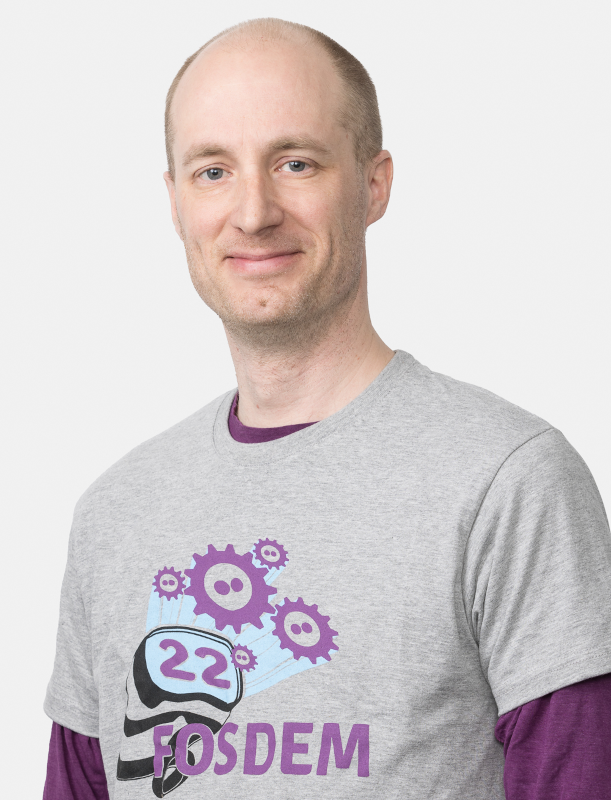
\includegraphics[width=1\linewidth]{img/me.png}
	\end{columns}
\end{frame}

%-------------- Powering a processor page

%Arrow style for all of the drawings
\tikzstyle{arrow} = [thick,->,>=stealth]

%Large SOC/PSY boxes
\tikzstyle{psys} = [rectangle, rounded corners, minimum width=3cm, minimum height=3cm,text centered, text width=3cm, draw=black, fill=red!30]
\tikzstyle{socs} = [rectangle, rounded corners, minimum width=3cm, minimum height=3cm,text centered, text width=3cm, draw=black, fill=green!30]

\addtocounter{framenumber}{-1}
\begin{frame}[plain]
\section{What and Why is a PMIC?}
%\note{Following section aims to give an idea about What a PMIC is and Why PMICs are needed?}
\end{frame}

\begin{frame}[t]{Powering a processor}\vspace{4pt}

%\note{could be this simple. Just passive source}
\note{could be}
\begin{itemize}
	\item Processor and peripherals need power
	\item Can be as simple as a dummy DC power source with correct voltage
\end{itemize}


\vfill
\centering
\begin{minipage}[c]{.75\textwidth}
%  \flushright

\begin{tikzpicture}[node distance=5cm]
	\node (psy) [psys] {DC-source};
	\node (soc) [socs, right of=psy] {SOC};
	\draw [arrow] (psy) -- node[anchor=south] {+5V} (soc);
\end{tikzpicture}
\end{minipage}
\end{frame}

%-------------- Powering a modern SOC page

%Small PSY clk and SOC boxes
%\tikzstyle{s_psys} = [rectangle, rounded corners, minimum width=2cm, minimum height=0.5cm,text centered, text width=2cm, draw=black, fill=red!30]
\tikzstyle{s_psys} = [rectangle, rounded corners, minimum width=2cm, minimum height=0.4cm,text centered, text width=2.5cm, draw=black, fill=red!30]
%\tikzstyle{s_clk} = [rectangle, rounded corners, minimum width=2cm, minimum height=0.5cm,text centered, text width=2cm, draw=black, fill=orange!40]
\tikzstyle{s_clk} = [rectangle, rounded corners, minimum width=2cm, minimum height=0.4cm,text centered, text width=2.5cm, draw=black, fill=orange!40]
\tikzstyle{s_socs} = [rectangle, rounded corners, minimum width=2.5cm, minimum height=3cm,text centered, text width=2.5cm, draw=black, fill=green!30]

\begin{frame}{Powering a modern SOC 1/2}

\note[item]{almost a real SOC.}
\note[item]{picture omits state GPIOs}
\note[item]{RTC clk}

	\begin{columns}[onlytextwidth]
	\column{0.22\linewidth}

	 Modern SOCs can require multiple specific voltages

	\column{0.75\linewidth} \vspace{4pt}

	\begin{tikzpicture}[node distance=0.52cm]
		\node (nvcc_snvs) [s_psys] {LDO1 1.8V};
		\node (vdd_snvs) [s_psys, below of=nvcc_snvs] {LDO2 0.8V};
		\node (rtc_clk) [s_clk, below of=vdd_snvs] {RTC-CLK};
		\node (vdd_soc) [s_psys, below of=rtc_clk] {BUCK1 0.8V};
		\node (vdd_gpu) [s_psys, below of=vdd_soc] {BUCK5 0.9V};
		\node (vdd_phy) [s_psys, below of=vdd_gpu] {LDO4 0.9V};
		\node (vdd_arm) [s_psys, below of=vdd_phy] {BUCK2 0.9V};
		\node (imx8) [s_socs, right of=vdd_arm, xshift=5cm]{SOC};
		\node (vdda_dram) [s_psys, below of=vdd_arm] {LDO3 1.8V};
		\node (nvcc_1v8) [s_psys, below of=vdda_dram] {BUCK7 1.8V};
		\node (nvcc_dram) [s_psys, below of=nvcc_1v8] {BUCK8 1.1V};
		\node (nvcc_3v3) [s_psys, below of=nvcc_dram] {BUCK6 3.3V};
		\node (vdd_phy_1v2) [s_psys, below of=nvcc_3v3] {LDO6 1.2V};
		\node (ldo5) [s_psys, below of=vdd_phy_1v2] {LDO5 3.3V};
		\node (mux)[s_psys, below of=ldo5]{MUX 1.8$\_$3.3V};

		\node (mux_to)[right of=mux, xshift=6cm]{};

		\draw [arrow] (nvcc_snvs) node[anchor=south, xshift=3cm] {\scriptsize NVCC-SNVS} -|  ([xshift=1.6cm] imx8);
		\draw [arrow] (vdd_snvs) node[anchor=south, xshift=3cm] {\scriptsize VDD-SNVS} -| ([xshift=0.5cm] imx8);
		\draw [arrow] (rtc_clk) node[anchor=south, xshift=3cm] {\scriptsize RTC-CLK} -| ([xshift=-0.5cm] imx8);
		\draw [arrow] (vdd_soc) node[anchor=south, xshift=3cm] {\scriptsize VDD-SOC-VDDA-PHY} -| ([xshift=-1cm] imx8);
		\draw [arrow] (vdd_gpu) -- node[anchor=south]{\scriptsize VDD-GPU-VPU-VRAM} (imx8.west|-vdd_gpu) ;
		\draw [arrow] (vdd_phy) -- node[anchor=south] {\scriptsize VDD-PHY} (imx8.west|-vdd_phy);
		\draw [arrow] (vdd_arm) -- node[anchor=south] {\scriptsize VDD-ARM} (imx8.west|-vdd_arm);
		\draw [arrow] (vdda_dram) -- node[anchor=south] {\scriptsize VDDA-DRAM-VDDA} (imx8.west|-vdda_dram);
		\draw [arrow] (nvcc_1v8) -- node[anchor=south] {\scriptsize NVCC} (imx8.west|-nvcc_1v8);
		\draw [arrow] (nvcc_dram) node[anchor=north, xshift=3cm] {\scriptsize NVCC-DRAM} -| ([xshift=-1cm] imx8);
		\draw [arrow] (nvcc_3v3) node[anchor=north, xshift=3cm] {\scriptsize NVCC-3V3} -| ([xshift=-0.5cm] imx8);

		\draw [arrow] (vdd_phy_1v2) node[anchor=north, xshift=3cm] {\scriptsize VDD-PHY-1V2} -| ([xshift=0.5cm] imx8);
		\draw [arrow] (ldo5) node[anchor=north, xshift=3cm] {\scriptsize LDO5-OUT} -| ([xshift=1.6cm] imx8);
		\draw [arrow](mux) node[anchor=north, xshift=3cm] {\scriptsize SD-CARD} -- (mux_to);
	\end{tikzpicture}
	\end{columns}
\end{frame}

%\begin{frame}[t]{Powering a modern SOC 1/2}\vspace{4pt}
%	\begin{columns}[onlytextwidth]
%	\column{0.5\linewidth}
%
%	 Modern SOCs can require multiple specific voltages
%
%	\column{0.7\linewidth}
%	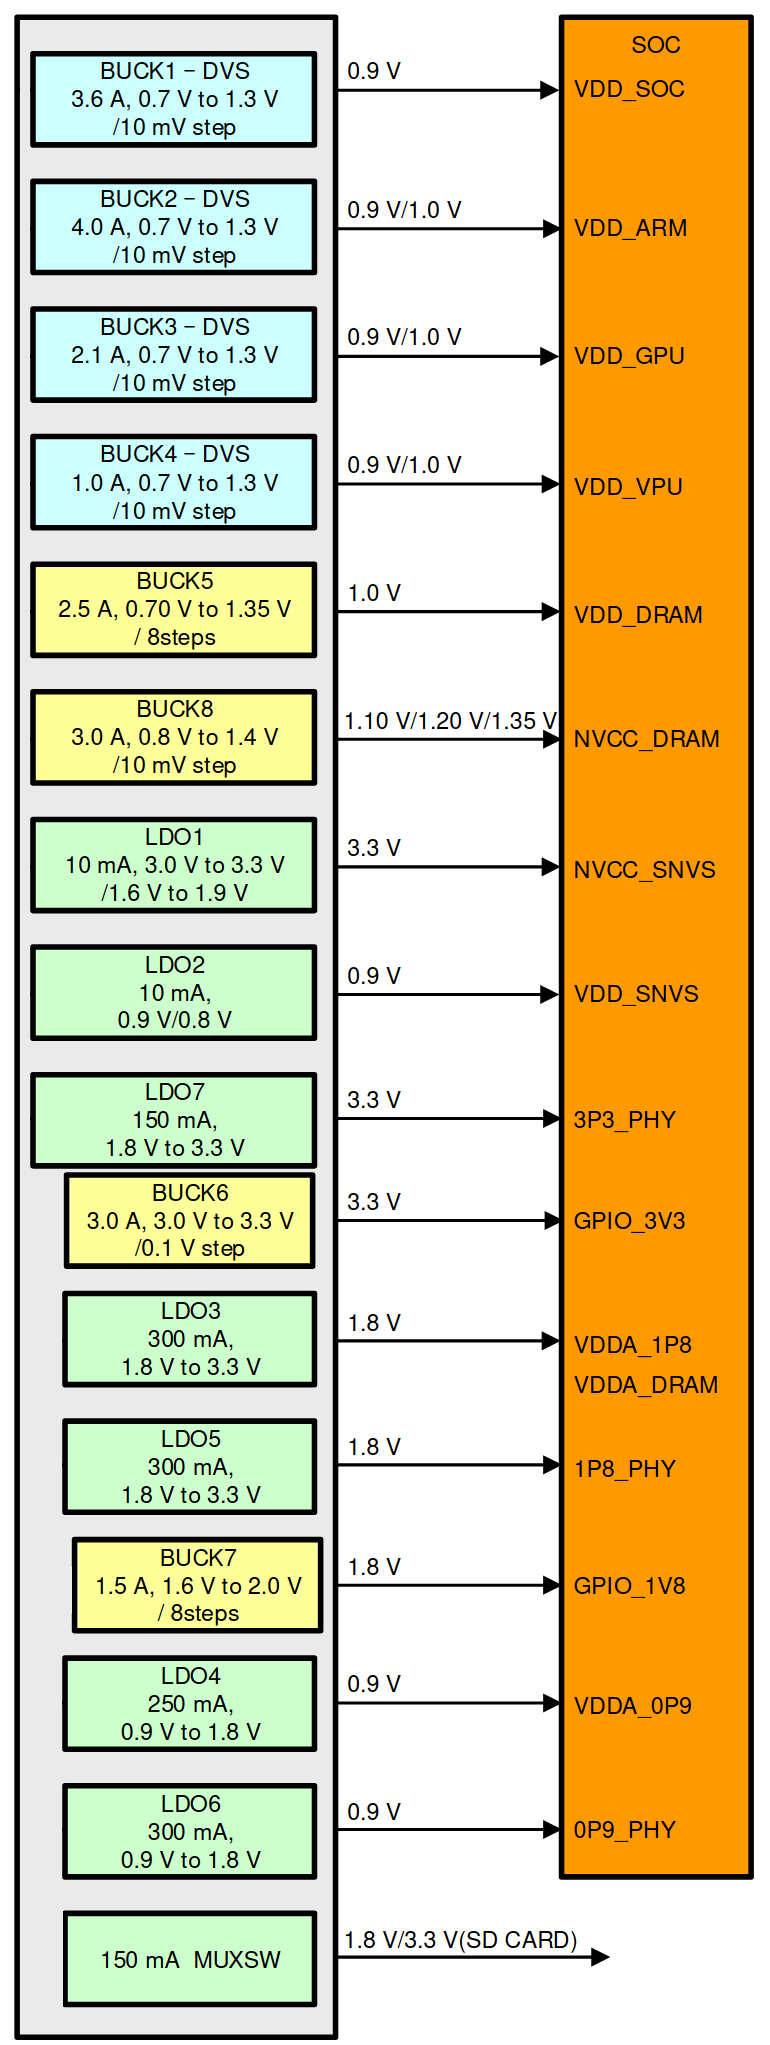
\includegraphics[width=0.4\linewidth]{img/imx8_power.png}
%	\end{columns}
%
%\end{frame}

%\begin{frame}[t]{Powering a modern SOC 1/2}%\vspace{4pt}
%	\begin{columns}[onlytextwidth]
%	\column{0.24\linewidth}
%
%	 Modern SOCs can require multiple specific voltages
%
%	\column{0.38\linewidth}
%	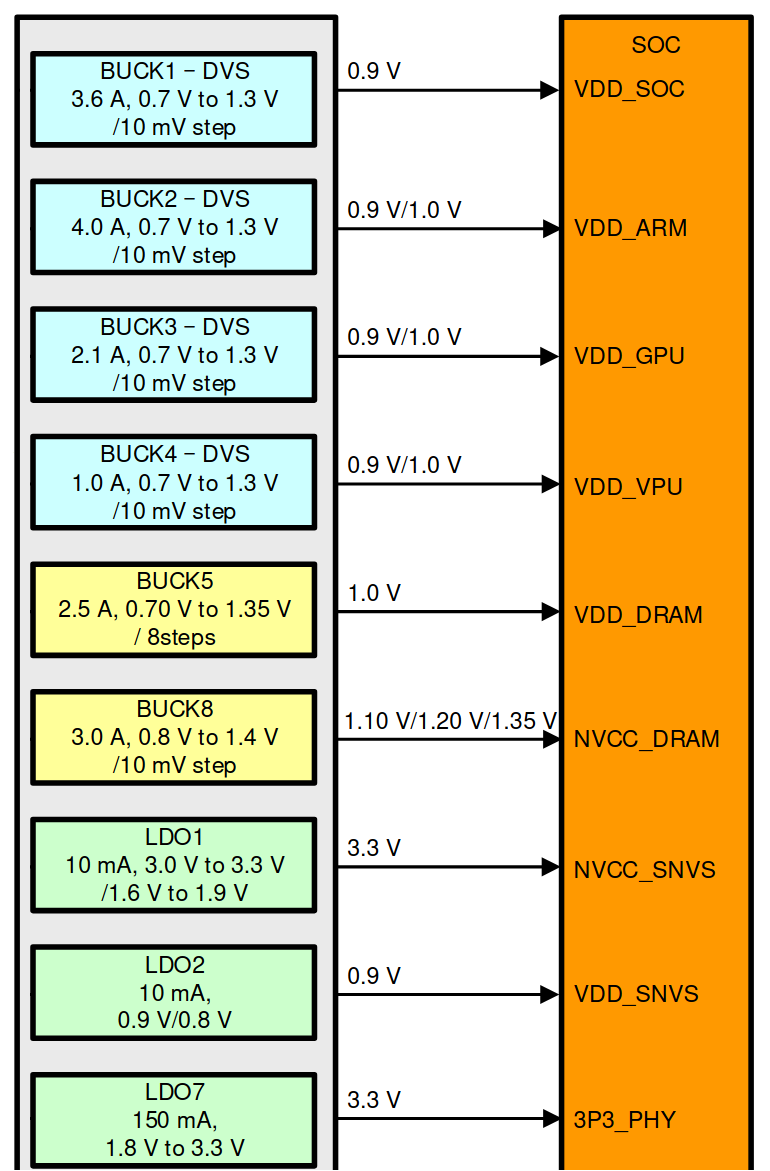
\includegraphics[width=1\linewidth]{img/imx8_power_split1.png}%\vspace{20pt}
%	\center continues ...
%	\column{0.38\linewidth}\vspace{50pt}
%	\center ... continues \\[12pt]
%	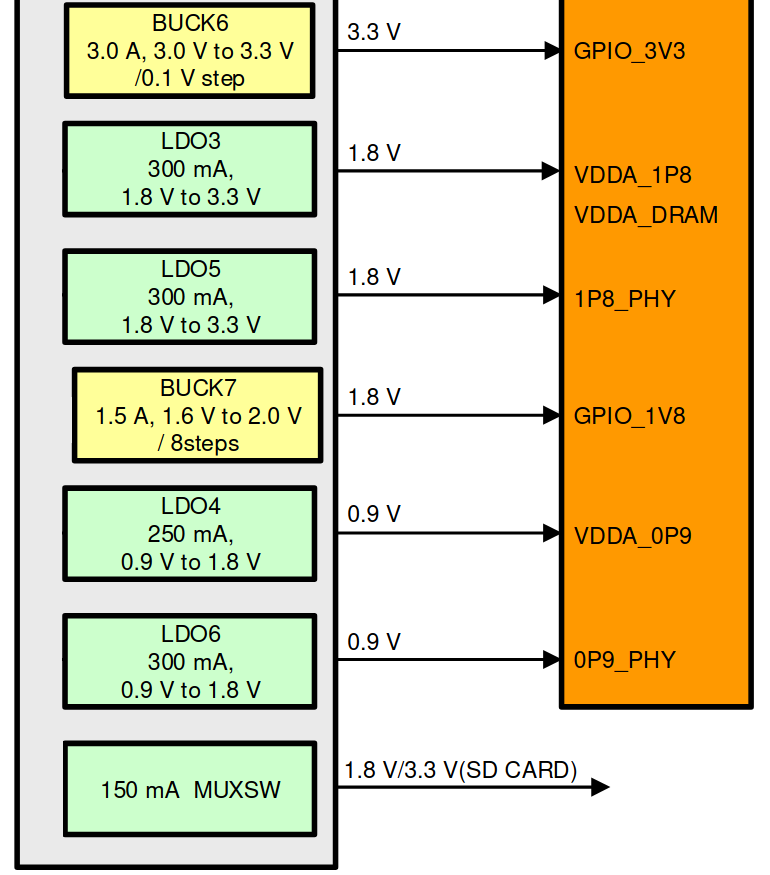
\includegraphics[width=1\linewidth]{img/imx8_power_split2.png}
%	\end{columns}
%
%\end{frame}


%-------------- Powering a modern SOC page 2

\begin{frame}{Powering a modern SOC 2/2}
\note[item]{TIMINGs - explain state transitions}
\note[item]{from PMIC spec}
\note[item]{shows also internal changes}
\note[item]{PCB area w/ discrete components}
\note[item]{New design for each  board(?)}
	\begin{columns}[onlytextwidth]
	\column{0.18\linewidth}
		And specific timings...
	\column{0.82\linewidth}\vspace{4pt}
		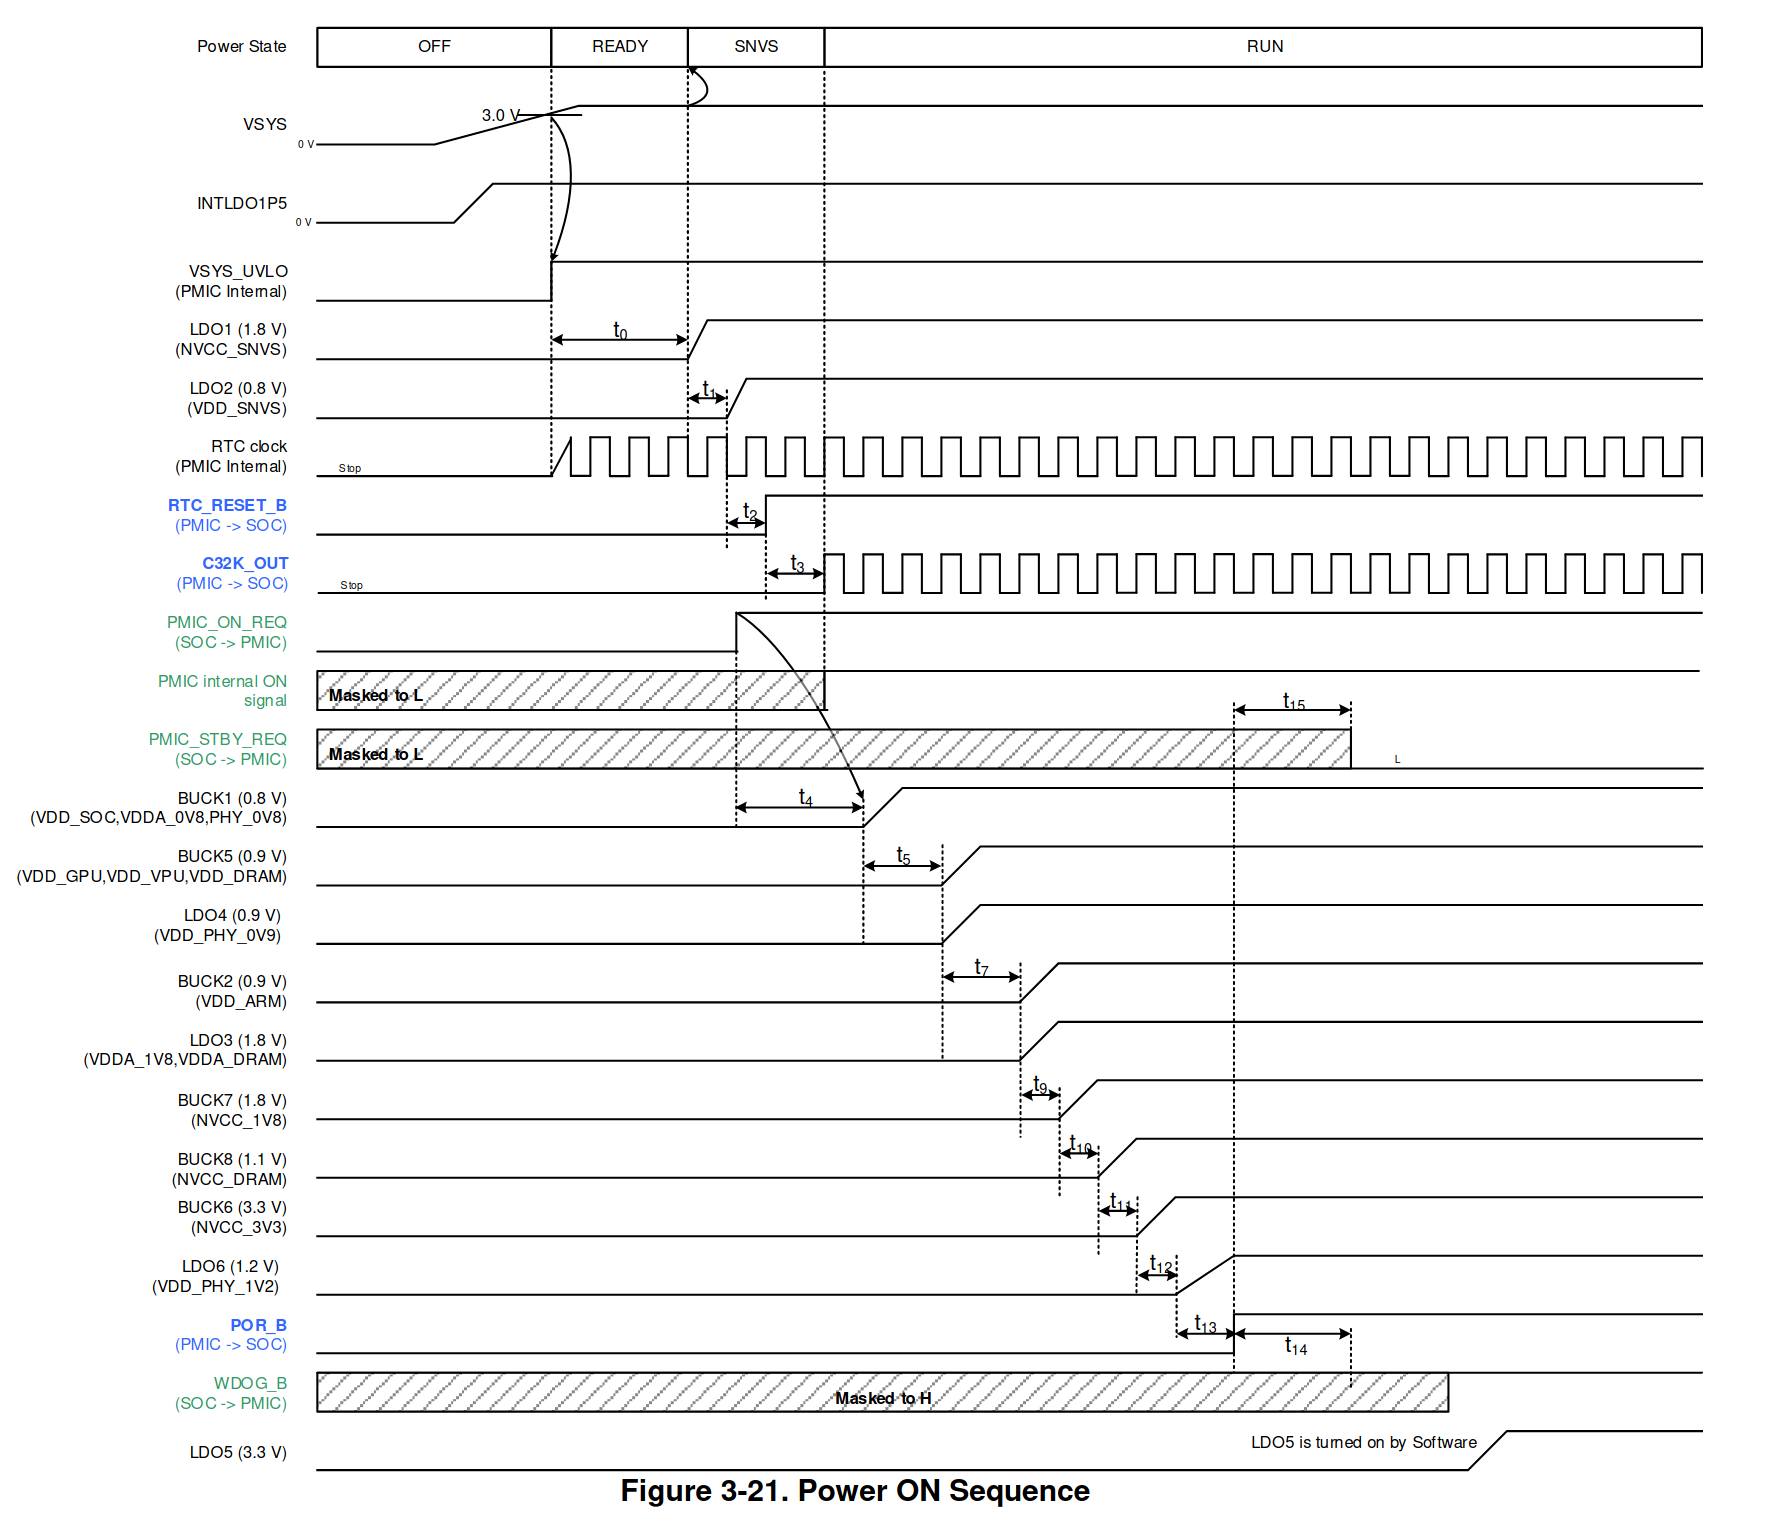
\includegraphics[width=1\linewidth]{img/BD71847_start_up_seq.png}
	\end{columns}
\end{frame}

%-------------- More control page

\begin{frame}{More control...}

\note[item]<1>{Importance of power saving increases}
\note[item]<1>{example: unused video-accelerator off}
\note[item]<1>{temperature}
%\note[item]{Changing voltages}
\note[item]<1>{Predefined states changed by GPIO (avoid I2C shut-down races I2C depends on some other block - other can't be shut down?)}

Power savings by:
\begin{itemize}
	\item Shutting down not needed devices
	\item Stand-by state(s)
	\item DVS (Dynamic Voltage Scaling)
\end{itemize}
\pause

Powering-on a system at given time / by an event.
\note[item]<2>{Monitor turn-on  input when SOC is shut down}
\note[item]<2>{For example RTC / HALL sensor (lid) }
\begin{itemize}
	\item RTC
%\end{itemize}
%...Or by an event
%\begin{itemize}
	\item HALL sensor, ...
\end{itemize}
\pause

More functionality
\begin{itemize}
	\item Battery / charger
	\item Watchdog
	\item Functional-safety
	\begin{itemize}
		\item Voltage monitoring
		\item Current monitoring
		\item Temperature monitoring
	\end{itemize}
\end{itemize}
%\note{More needs}
\note[item]<3>{battery powered devices everywhere}
\note[item]<3>{Watchdog almost every device has it}
\note[item]<3>{I have a feeling the importance of func safety increasing}

\end{frame}

%--------------  Automated power-on page

%\begin{frame}{Automated power on}
%Powering-on a system at given time...
%\note[item]{Monitor turn-on  input when SOC is shut down}
%\note[item]{For example RTC / HALL sensor (lid) }
%\begin{itemize}
%	\item RTC
%\end{itemize}
%...Or by an event
%\begin{itemize}
%	\item HALL sensor, ...
%\end{itemize}
%\end{frame}

%--------------  More requirements page

%\begin{frame}{More requirements...}
%\begin{itemize}
%	\item Battery / charger
%	\item Watchdog
%	\item Functional-safety
%	\begin{itemize}
%		\item Voltage monitoring
%		\item Current monitoring
%		\item Temperature monitoring
%	\end{itemize}
%\end{itemize}
%\note{More needs}
%\note[item]{battery powered devices everywhere}
%\note[item]{Watchdog almost every device has it}
%\note[item]{I have a feeling the importance of func safety increasing}
%\end{frame}

%--------------  PMICs page

\newcommand\TBox[2][]{%
  \tikz\node[draw,minimum width=1.8cm,minimum height=1cm,text centered,rounded corners,ultra thick,align=center,#1] {#2};}

\begin{frame}{PMICs}

\note[item] {PMICs created to support previous use-cases}
\note[item] {Often SOC specific}
\note[item] {also generic ones - very customizable (amount of outputs, voltages, sequences, state change controls (I2C, GPIO))}

PMIC - Power Management Integrated Circuit
\begin{itemize}
	\item Multiple DC sources with specific start-up / shut-down sequence
	\item Voltage control
	\item Functional-safety
	\item Auxiliary blocks to support various needs\\ [10pt]
\end{itemize}
\center
\TBox[fill=gray!30]{%
	\TBox[fill=red!30]{Regulators/Monitoring} PMIC \TBox[fill=cyan!30]{Battery/Charger} \\ [4pt]
	\TBox[fill=green!30]{Watchdog}\TBox[fill=green!30]{RTC}\TBox[fill=green!30]{CLK}\TBox[fill=green!30]{GPIO}} \\

%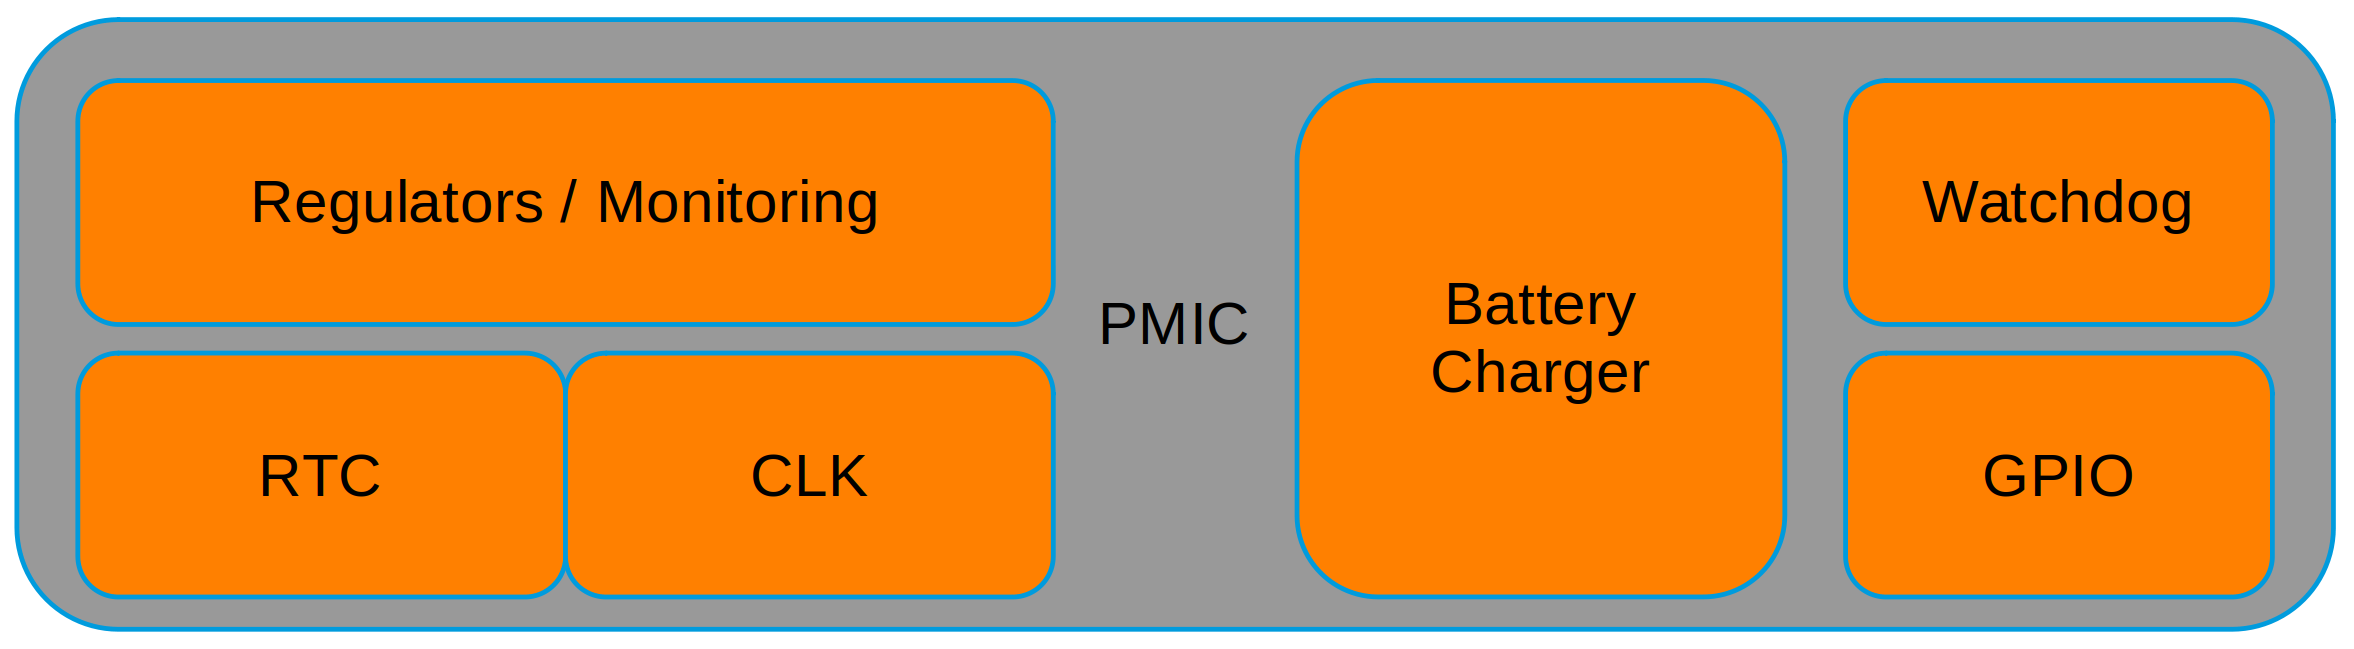
\includegraphics[width=1\linewidth]{img/pmic_block.png}
\end{frame}

%============== Section PMIC drivers

\addtocounter{framenumber}{-1}
\begin{frame}[plain]
\note[item]{What some typical PMIC drivers look like}
\note[item]{MFD}
\note[item]{Regulators}

\section{PMIC drivers}
\subsection{MFD and sub-devices}
\subsection{Regulators}
\end{frame}

%--------------  MFD page

\begin{frame}[t]{Multi Function Devices}
	\begin{columns}
	\column[t]{0.3\linewidth}
\begin{block}{Often MFD drivers}
%	\note[item]<1>{MFD "core" driver (Lee says there is no such "thing" as MFD)}
%	\note[item]<1>{core driver often provides bus access and IRQ controller code}
%	\note[item]<1>{core driver is created as any "standard driver" on that bus}
%	\note[item]<1>{Sub devices are (seemingly independent) platform devices}
%	\note[item]<1>{mfd-cell array describes sub-devices (drivers)}
%	\note[item]<1>{mfd registration instantiates sub-devices and runs driver probes}
%	\note[item]<1>{MODALIAS for module loading}
%	\note[item]<1>{Ask why MFD? (spoiler, re-use)}

	\note[item]<1>{"core" driver (Lee says there is no such "thing" as MFD)}
	\note[item]<1>{bus access and IRQ controller code}
	\note[item]<1>{core driver "standard driver" on that bus}
	\note[item]<1>{Sub devices independent platform devices}
	\note[item]<1>{mfd-cell array describes sub-devices (drivers)}
	\note[item]<1>{mfd registration instantiates sub-devices and runs driver probes}
	\note[item]<1>{MODALIAS for module loading}
	\note[item]<1>{Ask why MFD? (spoiler, re-use)}

%	\note[item]<2>{Many devices re-use digital blocks from previous generations while adding something new}
%	\note[item]<2>{MFD sub-devices can be re-used and new drivers written only for new blocks (ideally)} 
	\note[item]<2>{HW re-use digital blocks from previous generations}
	\note[item]<2>{MFD sub-devices can be re-used and new drivers written only for new blocks (ideally)} 
	\begin{itemize}
		\item \textbf{Regulator}
		\item RTC
		\item Power supply
		\item Watchdog
		\item GPIO
		\item CLK ...
	\end{itemize}
\end{block}
	\column[t]{0.68\linewidth}
		%\only<1> {\textbf{Why?} (I have 1 reason on mind, may be more)}
		\only<1>{
			\textbf{Why?} (I have 1 reason on mind, may be more)
			%\textbf{Allows re-use \\[10pt]}
			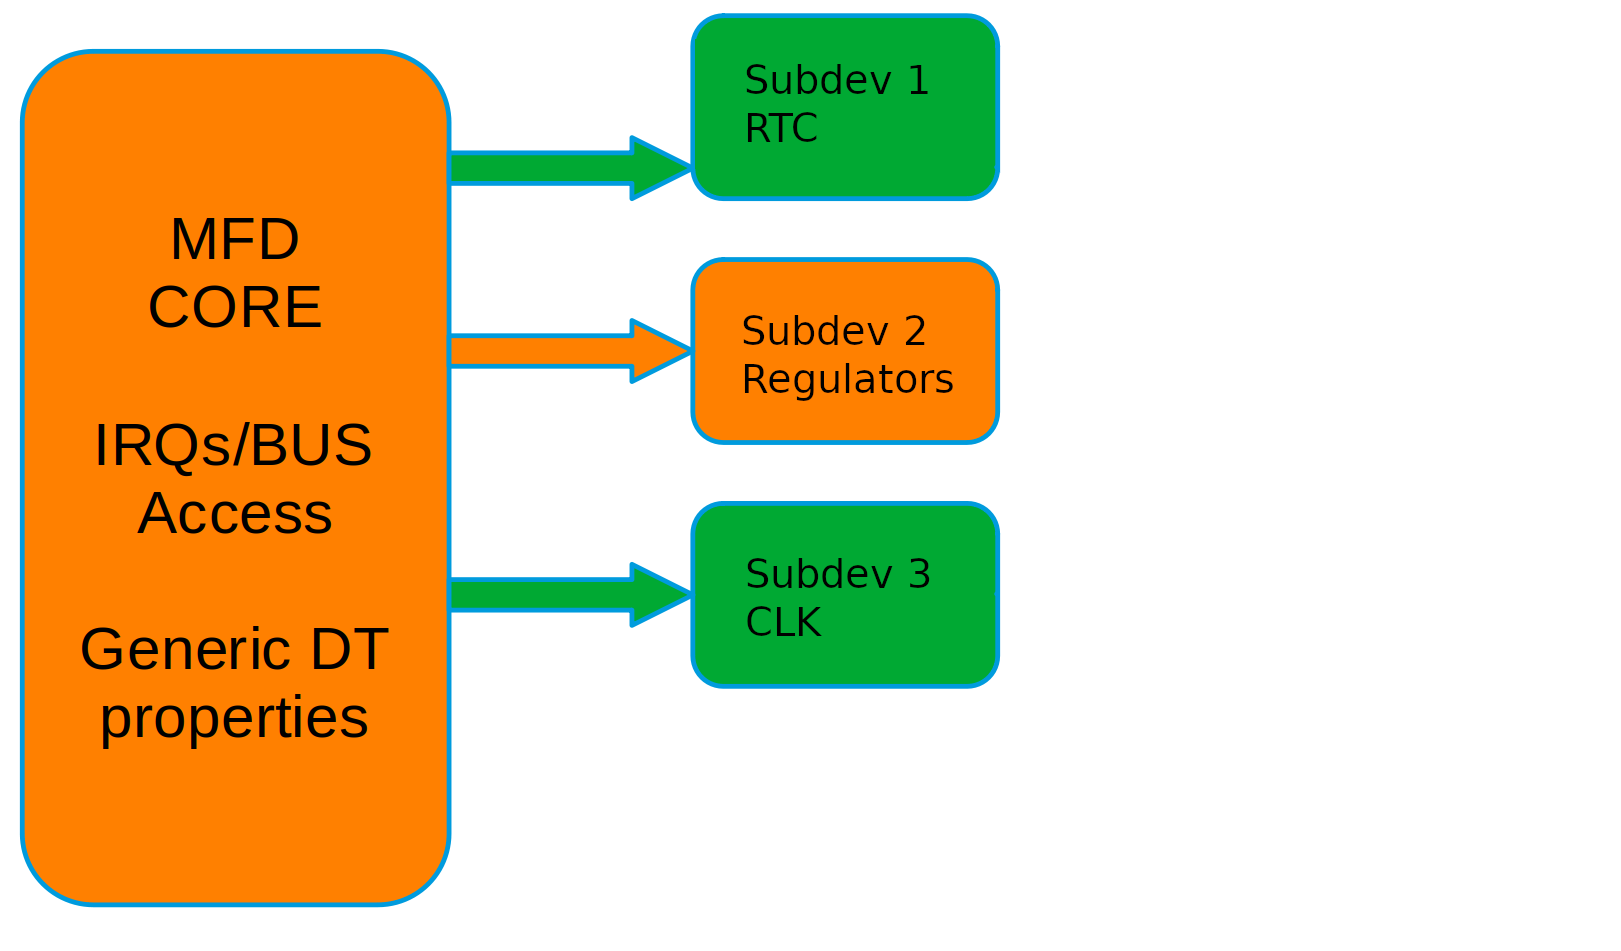
\includegraphics[width=1\linewidth]{img/MFD_re_use1.png}
		}
		\only<2>{
			\textbf{Allows re-use \\[10pt]}
			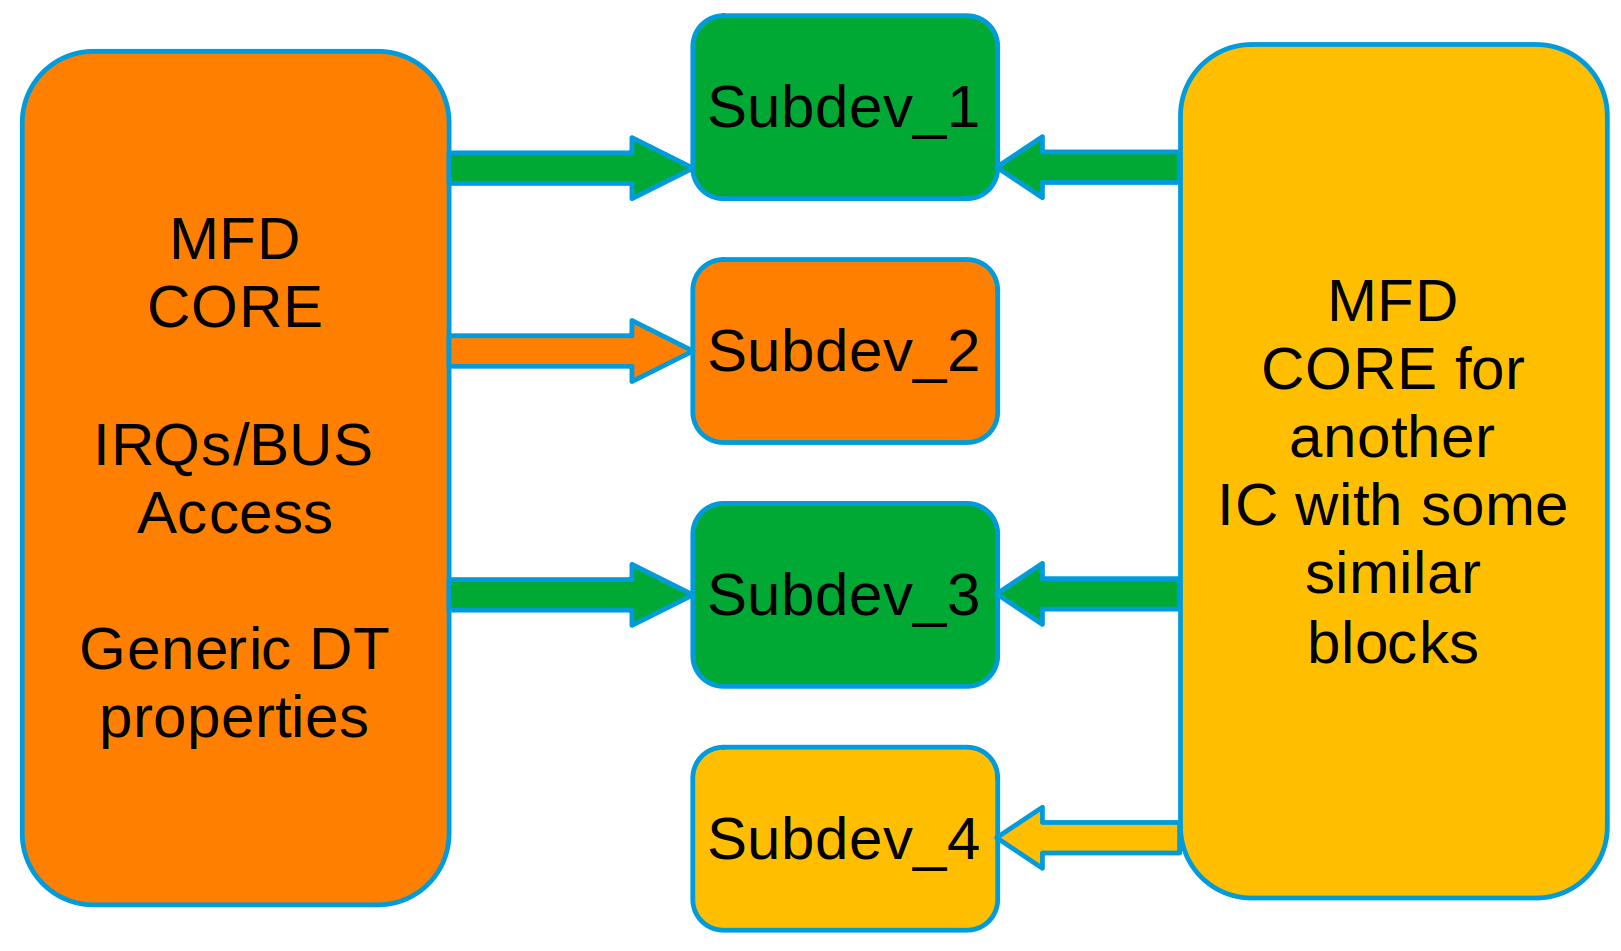
\includegraphics[width=1\linewidth]{img/MFD_re_use.png}
		}
	\end{columns}
\end{frame}

%--------------  regulator consumer/provider page

\begin{frame}[t]{Regulator (provider) and consumer}\vspace{4pt}

\note[item]{framework between hardware driver - user}
\note[item]{regulator API to consumers}
\note[item]{framework -\textgreater driver -\textgreater PMIC regs}
\note[item]{example, sensor driver}
\note[item]{request enable via regulator API}
\note[item]{regulator framework calls callbacks from regulator driver}

\begin{itemize}
	\item Provider is driver interfacing the hardware. Eg, sits “below” the regulator framework. Between regulator framework and HW
	\item Consumer is driver who wishes to control the regulator using the regulator framework. Eg, sits “on top of” the regulator framework
	\item PMIC driver is the provider driver (usually just referred as a regulator driver) \\[10pt]
\end{itemize}
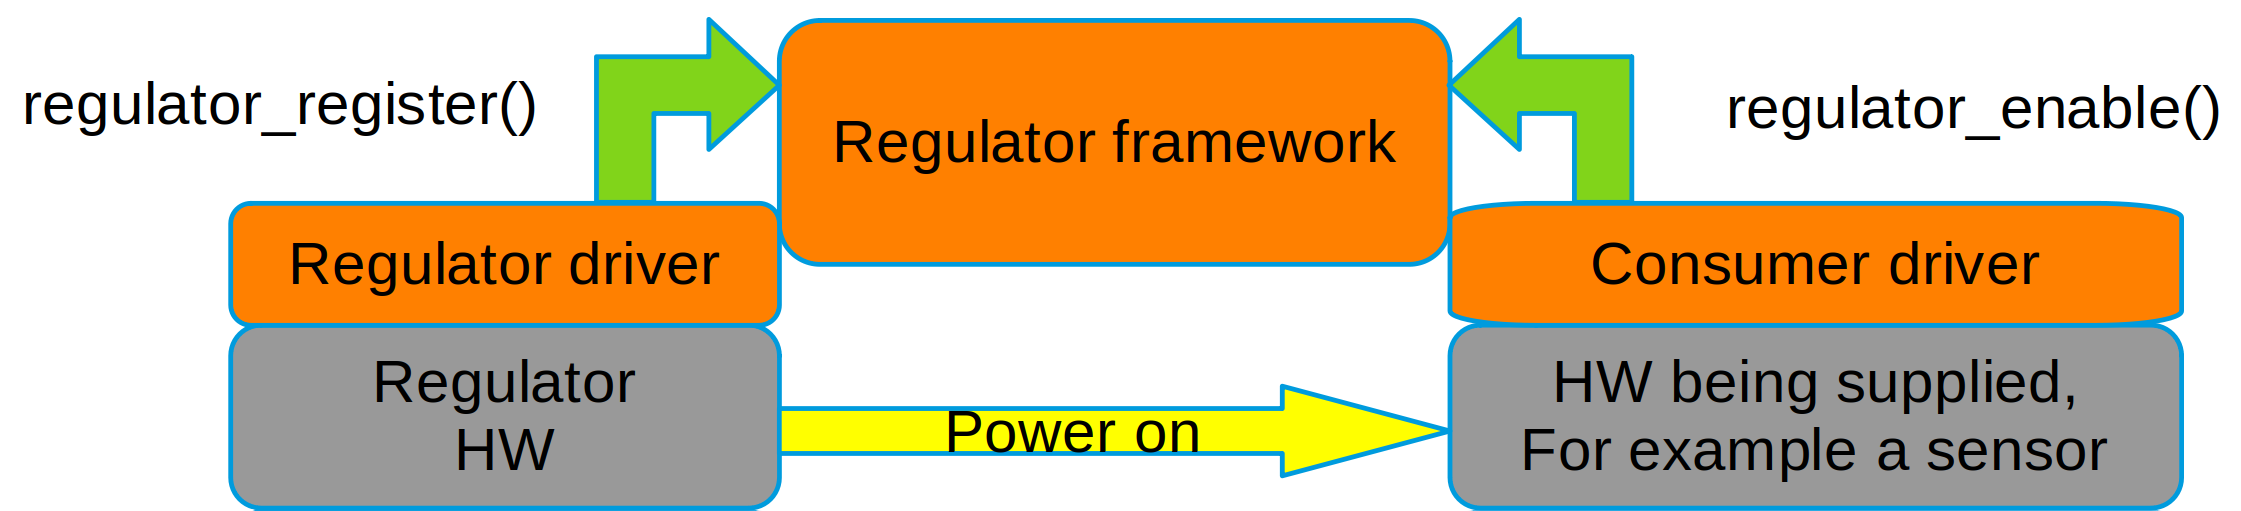
\includegraphics[width=1\linewidth]{img/regulator_users.png}
\end{frame}

\newcommand{\mycfile}[1]{\textit{\small #1}}

%-------------- Regulator ops

\begin{frame}[fragile, t]{Regulator driver ops}\vspace{4pt}
\begin{block}{Regulator driver relies on callbacks}
Regulator (provider) registers callbacks to regulator framework.
Framework handles regulators using these ops.
\end{block}

\mycfile{include/linux/regulator/driver.h}
\lstset{language=C}
\scriptsize
\begin{lstlisting}
struct regulator_ops {
	// snip
	int (*enable) (struct regulator_dev *);
	int (*disable) (struct regulator_dev *);
	int (*is_enabled) (struct regulator_dev *);
	int (*set_voltage_sel) (struct regulator_dev *, unsigned selector);
	int (*get_voltage_sel) (struct regulator_dev *);
	// snip
};
\end{lstlisting}
\pause

\begin{lstlisting}
struct regulator_desc {
	/* Plenty of regulator properties */
	/* Also information for the helpers */
	/* Finally the ops */
	const struct regulator_ops *ops;
}
\end{lstlisting}
\end{frame}

%-------------- Regulator constraints

\begin{frame}[t]{Regulator constraints}\vspace{4pt} 
\begin{block}{Regulators can have constraints.}
Not to be mixed with limits discussed during the rest of the presentation.
\end{block}
\par
\begin{columns}
\column[]{0.72\linewidth}
\begin{itemize}
	\item struct regulation$\_$constraints \mycfile{include/linux/regulator/machine.h}
	\item hard limits forced by the regulator framework.
	\item can be given by driver in dynamic init data
	\item can be given via device-tree
	\item voltage / current range, prevent disabling, step size ...
\end{itemize}
\column[]{0.28\linewidth}
%width=1\linewidth
\begin{figure}

\includegraphics[height=0.55\textheight]{image_dl/stopman.jpg}
\scriptsize Image: \thinspace{\itshape Peggy und Marco Lachmann-Anke, Pixabay}
\end{figure}
\end{columns}
\end{frame}
%============== Section Functional-safety

\addtocounter{framenumber}{-1}
\begin{frame}[plain]
%\note[item]{rest of the show explains how regulator framework can be used to deliver errors. From PMIC vendor perspective - sorry}
\note[item]{how regulator framework can be used to deliver errors}
\note[item]{ From PMIC vendor perspective - sorry}
\section{Monitoring for abnormal conditions}
\subsection{Severity levels and limit values}
\subsection{Regulator errors and notifications}
\subsection{Helpers and examples}
\begin{figure}
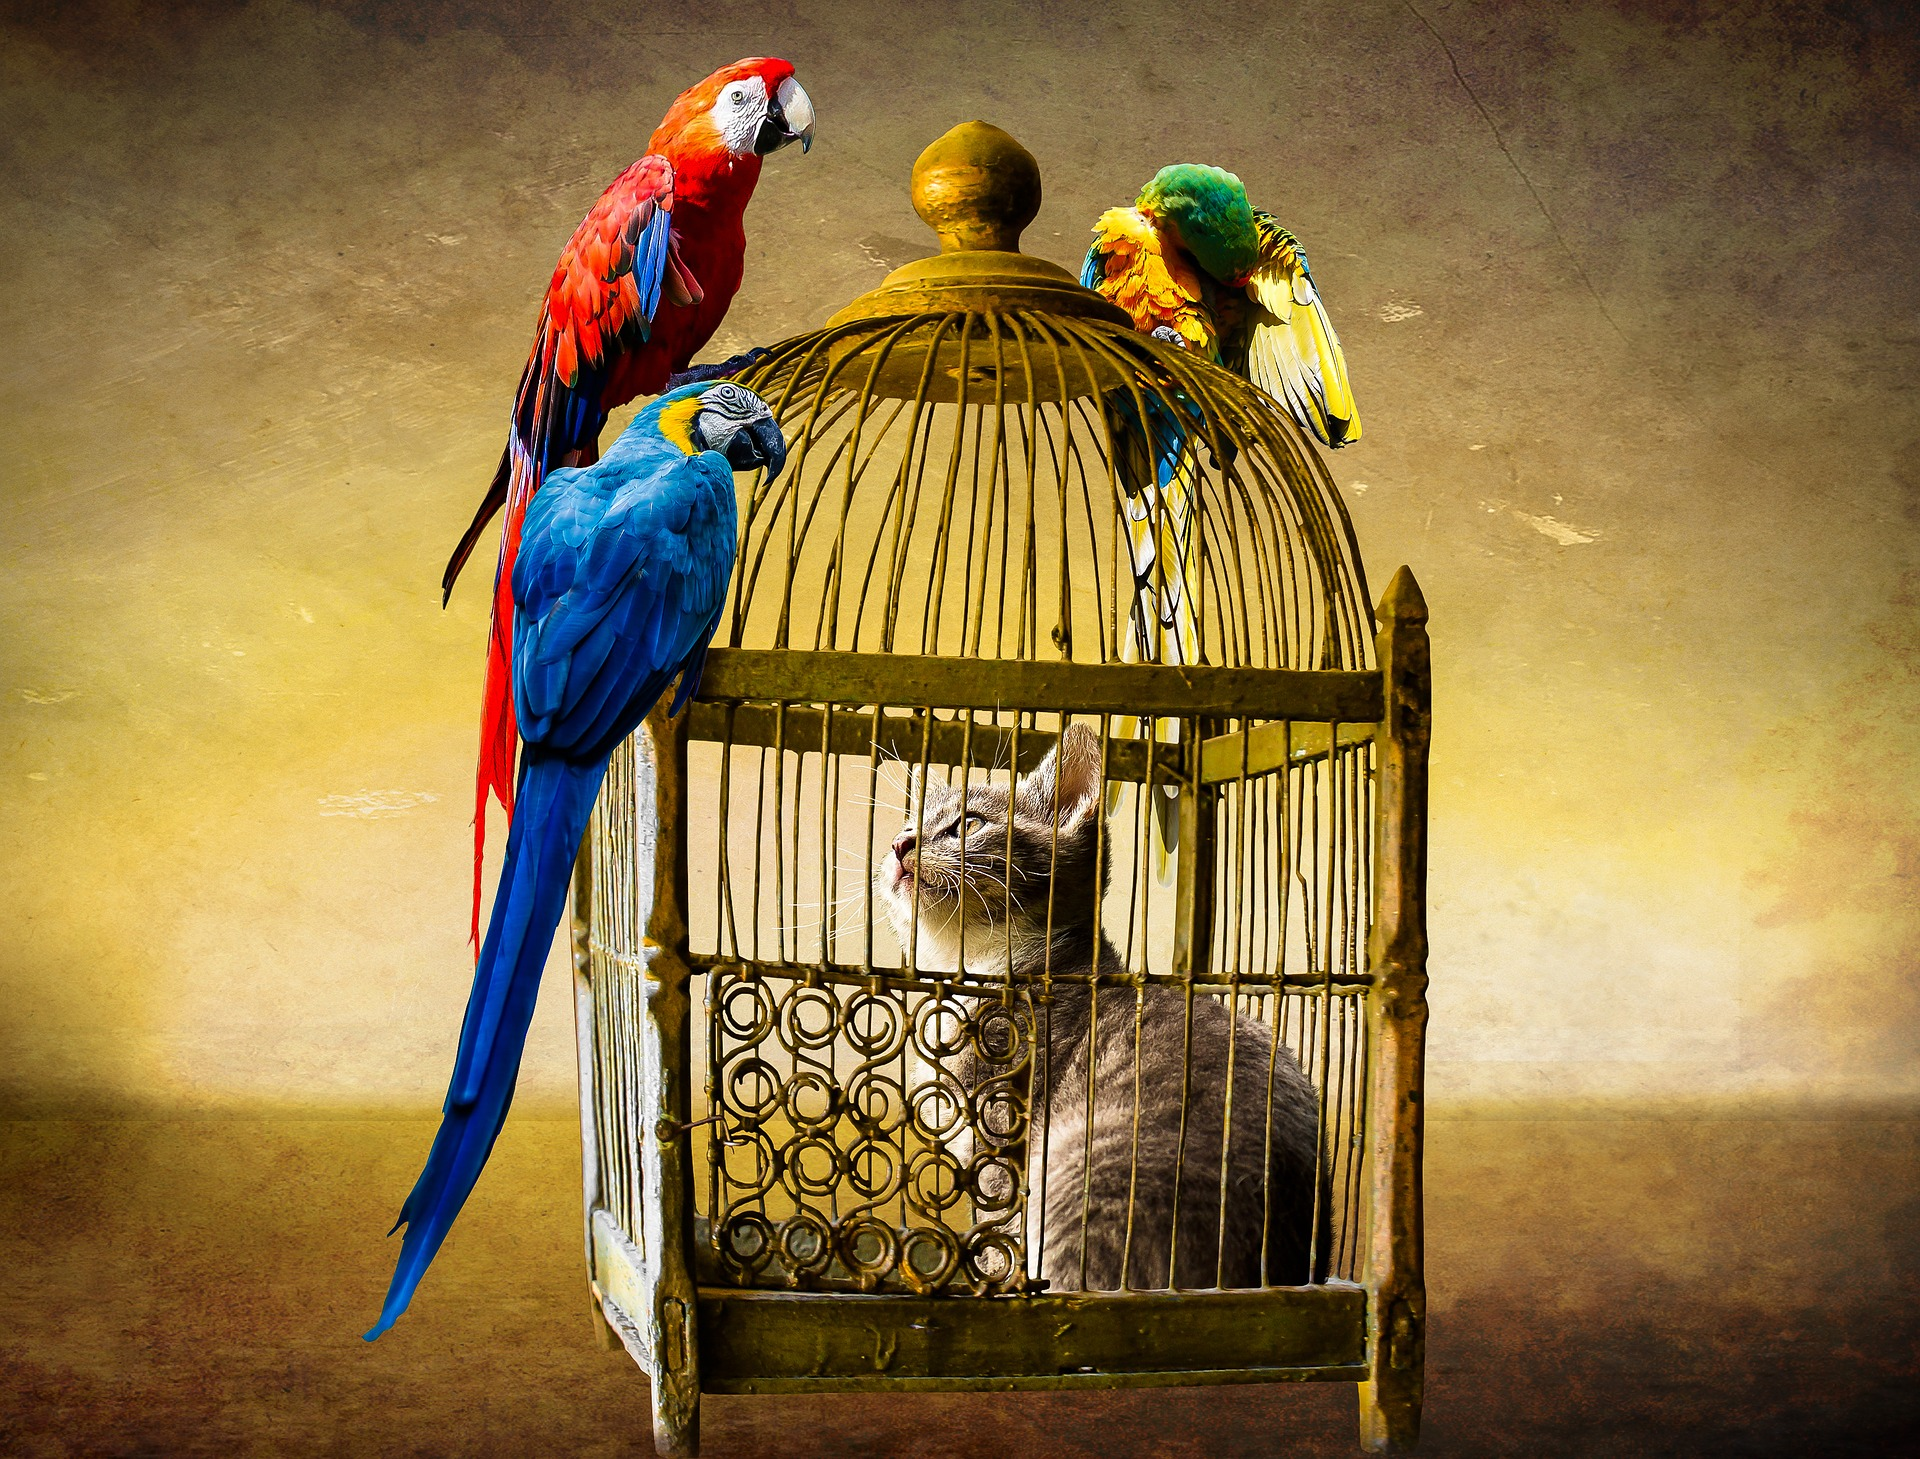
\includegraphics[scale=0.36]{image_dl/kissa-hakissa.jpg} \\
\scriptsize Image: \thinspace{\itshape Gerhard, Pixabay}
\end{figure}
\end{frame}


%-------------- notification / error flags page

\begin{frame}[t]{Detecting unexpected}\vspace{4pt}

%	\note[item]<2>{PROTECTION example, severe over-voltage - PMIC shuts down all or offending outputs}
%	\note[item]<2>{Could be also temperature-error or over-current}
\note[item]<2>{severe over-voltage}
\note[item]<2>{temperature-error, over-current}

%\note[item]<3>{Some PMICs may not automatically shut down outputs - SW should do it}
%\note[item]<3>{ERROR still indicate fatal issues - HW not working}

\note[item]<3>{Some PMICs do not automatically shut down outputs - SW should do it}
\note[item]<3>{still fatal issues - HW not working}

%\note[item]<4>{WARNING included in kernel 5.14}
%\note[item]<4>{Intended to be used for invoking corrective action(s)}
%\note[item]<4>{Has been requested from us - there probably are use-cases}
%\note[item]<4>{I have no insight as to what they could be - very interested in learning any concrete examples - ask from audience}

\note[item]<4>{in kernel 5.14}
\note[item]<4>{for invoking corrective action(s)}
\note[item]<4>{Has been requested from us - there probably are use-cases}
\note[item]<4>{No insight or concrete examples - ask from audience}

\begin{block}{Linux has 3 severity categories}
%\begin{itemize}
The categories - PROTECTION, ERROR, WARNING - inform the hardware state.
%\end{itemize}
\end{block}

%\begin{itemize}
\onslide<2>{
%	\item  \textbf{PROTECTION}
\textbf{PROTECTION}
	\begin{itemize}
		\item Unconditional \textcolor{magenta}{shutdown by HW}
	\end{itemize}
}

\onslide<3>{
%	\item \textbf{ERROR}
	\textbf{ERROR}
	\begin{itemize}
		\item \textcolor{red}{Irrecoverable error,} system not expected to be usable. Error handling by software.
	\end{itemize}
}
\onslide<4>{
%	\item  \textbf{WARNING} - NEW(ish)
	\textbf{WARNING} - NEW(ish)
	\begin{itemize}
		\item \textcolor{orange}{Something is off-limit,} system still usable but a recovery action should be taken to prevent escalation to errors
%	\end{itemize}
}

\end{itemize}
\end{frame}

%--------------  setting safety limits via device-tree page

\begin{frame}[t]{Safety limits, device-tree}\vspace{4pt}

%\note[item]<1>{Often board specific - Can be provided via device-tree}
\note[item]<1>{Board specific -\textgreater via device-tree}
\note[item]<1>{property format from box}

%\note[item]<2>{value sets new limit}
%\note[item]<2>{1 / 0 special values - they are used to indicate enable / disable}
\note[item]<2>{explain values, pause}

\onslide<1-2>{
\begin{block}{Property format:}
\begin{itemize}
	\item  regulator-\textless event \textgreater-\textless severity \textgreater-\textless unit \textgreater = value
\end{itemize}
\end{block}

Over current:
\begin{itemize}
	\item regulator-oc-protection-microamp
	\item regulator-oc-error-microamp
	\item regulator-oc-warn-microamp
\end{itemize}

Similar for over voltage (ov), under voltage (uv) and temperature (temp)
}
\onslide<2>{
\par
Values:
\begin{itemize}
	\item 0 =\textgreater disable
	\item 1 =\textgreater enable
	\item other =\textgreater new limit
\end{itemize}
}
\end{frame}

\addtocounter{framenumber}{-1}
\begin{frame}[t]{Safety limits, device-tree}\vspace{4pt}
\note[item]{I have no good answer.}
\note[item]{Ask, What happens if silently ignored?}
\note[item]{Ask, What happens if regulator registration fails?}
\note[item]{/* If limit is silently ignored - problems for example when changing a component and new driver does not support limits */}
\note[item]{/* If registration fails, system may not boot, boot without display etc. */}
\normalsize
\note[item]{Currently just log a warning}
\note[item]{In general, is there a way to mark NOT supported properties to binding docs? Would it help? Including ALL regulator bindings does hide this at a validation stage}
\note[item]{pause}
\note[item]{I know you are eager to see the code :) So, let's look at some}
\center
%\textcolor{red}{\textbf{What if hardware does not support given limit?}}
\large \textbf{What if hardware does not support given limit?}
\begin{figure}

\includegraphics[scale=0.30]{image_dl/question.png} \\
\scriptsize Image:\thinspace{\itshape Pete Linforth, Pixabay}
\end{figure}
\end{frame}

%--------------  limit config callbacks page


\begin{frame}[fragile]{Callbacks for configuring the limits}
\note[item]<1>{Callbacks for over-current, over- and under-voltage, over temperature}
\note[item]<1>{Arguments include the limit, severity (PROT, ERR, WARN) and enable/disable}
\note[item]<2>{Callbacks are among the other regulator ops which is pointed from the regulator description}
\note[item]<3>{The description with ops is passed to regulator registration}

%\textbf{Regulator framework interface:}\vspace{4pt}

%\small include/linux/regulator/driver.h
%\small \textit{include/linux/regulator/driver.h}
\mycfile{include/linux/regulator/driver.h}
\lstset{language=C}
\scriptsize
\begin{lstlisting}
struct regulator_ops {
	// snip
	int (*set_over_current_protection)(struct regulator_dev *,
	       int lim_uA, int severity, bool enable);
	int (*set_over_voltage_protection)(struct regulator_dev *,
	      int lim_uV, int severity, bool enable);
	int (*set_under_voltage_protection)(struct regulator_dev *,
	     int lim_uV, int severity, bool enable);
	int (*set_thermal_protection)(struct regulator_dev *,
	     int lim, int severity, bool enable);
};
\end{lstlisting}
\pause

\begin{lstlisting}
struct regulator_desc {
	// snip
	const struct regulator_ops *ops;
};
 \end{lstlisting}
\pause

\begin{lstlisting}
struct regulator_dev *devm_regulator_register(struct device *dev,
		const struct regulator_desc *regulator_desc,
		const struct regulator_config *config);
\end{lstlisting}
\end{frame}

%--------------  page limiting Example


\begin{frame}[fragile]{Simplified example}
\note[item]{Example of over-current protection example using pieces of ROHM BD9576 driver as example}
\note[item]{Regulator framework parses dt properties and invokes callback with values found from DT}
\note[item]{Driver typically checks for parameter sanity/support}
\note[item]{Driver decides the register and values to write based on severity and limit}
\note[item]{for example BD9576 has different register and limit ranges for warning and protection}
\note[item]{From the PMIC operation POV there is no difference between ERROR and WARNING}
\note[item]{Finally if limits were sane, the driver updates new limits to registers and returns Ok}

\mycfile{drivers/regulator/bd9576-regulator.c}

\lstset{language=C}
\scriptsize
\begin{lstlisting}[commentstyle=\color{orange}]
static int bd9576_set_ocp(struct regulator_dev *rdev, int lim_uA,
			  int severity, bool enable)
{
	...

	/* Return -EINVAL for unsupported configurations */
	if ((lim_uA && !enable) || (!lim_uA && enable))
		return -EINVAL;

	/*
	 * Select the correct register and appropriate register-value
	 * conversion for given severity and limit..
	 */
	if (severity == REGULATOR_SEVERITY_PROT) {
		...
	} else {
		...
	}

	/* Write configuration to registers */
	return bd9576_set_limit(range, num_ranges, d->regmap,
				reg, mask, Vfet);
}
\end{lstlisting}
\end{frame}

%--------------  informing the unexpected page

\begin{frame}[t]{Informing the unexpected}\vspace{4pt}
\note[item]<1>{So, when an abnormal event is detected by HW (something exeeds the limit) we need to inform consumers}
\note[item]<1>{The regulator framework can use ERRORs or NOTIFICATIONs}
\note[item]<1>{Errors visible via sysfs}
\note[item]<2>{Errors are simple status which is stored in framework}
\note[item]<2>{Errors need to be polled by consumers}
\note[item]<2>{Polling is not always preferred}
\note[item]<3>{Notifications are sent by HW when problem occurs}
\note[item]<3>{No polling needed - except to know when condition is back to normal}
\note[item]<3>{Not all notifications are errors...}

\begin{block}{Two types of information}
\begin{itemize}
	\item ERRORs
	\item NOTIFICATIONs
\end{itemize}
\end{block}

\begin{itemize}
\onslide<2->{
	\item  \textbf{ERROR}
	\begin{itemize}
		\item set by provider
		\item queried (polled) by consumer
		\item regulator$\_$get$\_$error$\_$flags()
	\end{itemize}
}
\onslide<3>{
	\item \textbf{NOTIFICATION}
	\begin{itemize}
		\item sent by provider (usually) from interrupt
		\item invoke consumer callback (blocking notifier call-chain)
		\item In some (many) cases IRQ is held active for whole duration of error
		\item no polling needed
		\item regulator$\_$register$\_$notifier()
		\item can send also other events
	\end{itemize}
}
\end{itemize}
\end{frame}

%--------------  list of errors page

\begin{frame}[fragile]{Regulator error flags}
\note[item]{The available ERROR definitions}
\note[item]{I've used REGULATION-OUT for over-voltage}
\note[item]{Not sure where REGULATOR-ERROR-FAIL is used}
\mycfile{include/linux/regulator/consumer.h}
\begin{lstlisting}
#define REGULATOR_ERROR_UNDER_VOLTAGE
#define REGULATOR_ERROR_OVER_CURRENT
#define REGULATOR_ERROR_REGULATION_OUT
#define REGULATOR_ERROR_FAIL
#define REGULATOR_ERROR_OVER_TEMP
#define REGULATOR_ERROR_UNDER_VOLTAGE_WARN
#define REGULATOR_ERROR_OVER_CURRENT_WARN
#define REGULATOR_ERROR_OVER_VOLTAGE_WARN
#define REGULATOR_ERROR_OVER_TEMP_WARN
\end{lstlisting}
\end{frame}

%--------------  list of notifications page

\begin{frame}[fragile]{Regulator notifications}
\note[item]{The available EVENT definitions}
\note[item]{Note, not all of the notificatin types listed as some are not failures}
\note[item]{Last one (WARN-MASK) is not event but a mask for consumers to allow checking if notification was a warning}
\mycfile{include/linux/regulator/consumer.h}
\begin{lstlisting}
#define REGULATOR_EVENT_UNDER_VOLTAGE 
#define REGULATOR_EVENT_OVER_CURRENT  
#define REGULATOR_EVENT_REGULATION_OUT
#define REGULATOR_EVENT_FAIL
#define REGULATOR_EVENT_OVER_TEMP
...
#define REGULATOR_EVENT_UNDER_VOLTAGE_WARN
#define REGULATOR_EVENT_OVER_CURRENT_WARN
#define REGULATOR_EVENT_OVER_VOLTAGE_WARN
#define REGULATOR_EVENT_OVER_TEMP_WARN
#define REGULATOR_EVENT_WARN_MASK
\end{lstlisting}

\end{frame}

%--------------  Notifications page

%\begin{frame}{Notifications}
%\note[item]{Usually an IRQ is generated by HW when error is observed}
%\note[item]{Regulator notifications use blocking call-chain, notifiers should fire from process context}
%\note[item]{Often the IRQ is held active for the duration of a problem}
%\note[item]{Need special handling to avoid IRQ storm which would not exactly help mitigating issues}
%\note[item]{The event executes the action registered by the consumer}
%Usually IRQ backed
%\begin{enumerate}
%	\item PMIC detects error and generates IRQ
%	\item IRQ handler sends notification
%	\item Regulator consumer action is executed
%\end{enumerate}
%\pause
%In some (many) cases IRQ is held active for whole duration of error
%\begin{itemize}
%	\item Maybe because these IRQs are considered as a last thing?
%	\item Maybe because there is need to ensure IRQ is not missed?
%	\item Does not play well with all systems
%\end{itemize}
%\end{frame}

%-------------- IRQ helper page

\begin{frame}[fragile, t]{Event IRQ helper}\vspace{4pt}
\note[item]{helper provided}
\note[item]{read the box}
\note[item]{helper is registered using below API - we will see it in more details later}
\begin{block}{A helper provided for IRQ handling and sending the notification}
\begin{itemize}
	\item Supports keeping IRQ disabled for a period of time
	\item Supports forcibly shutting down the system if accesing the PMIC fails
\end{itemize}
\end{block}
\vfill
\lstset{language=C}
\scriptsize
\begin{lstlisting}
void *regulator_irq_helper(struct device *dev,
		   const struct regulator_irq_desc *d, int irq,
		   int irq_flags, int common_errs, 
		   int *per_rdev_errs, struct regulator_dev **rdev,
		   int rdev_amount);
\end{lstlisting}
\end{frame}

%-------------- Helper break-out page

\begin{frame}[t]{Helper break-out}\vspace{4pt}
\note[item]<1>{But first, let's go through the helper operation}
\note[item]<1>{Box on the left represent functionality in helper}
\note[item]<1>{ellipse represent functionality implemented in driver}
\note[item]<1>{Let's walk through the notification process}

\note[item]<2>{abnormal event is detected by HW}
\note[item]<3>{helper runs ISR and calls map$\_$event() from driver to know what happened}
\note[item]<4>{map$\_$event() returns information about fatal access failure}
\note[item]<4>{If error was fatal, helper will call die() callback from driver or try execute emergency power-off}
\note[item]<4>{The die() callback can be used to provide emergency operation like turning off the failing power}
\note[item]<5>{Helper will send the notifications to consumers and update the error flags}
\note[item]<5>{Helper will schedule the IRQ re-enable}
\note[item]<6>{When it is time to re-enable the IRQ, helper will ask driver if problem is over and IRQ can be re-enabled}
\note[item]<7>{If IRQ can be re-enabled, the helper unmasks it. If not, the re-enable is scheduled again}
\begin{columns}[onlytextwidth]
	\column[t]{0.25\linewidth}
	events
	\only<2->{
		
\includegraphics[width=1\linewidth]{img/isr/IRQ.png}
	}
	\only<4->{
		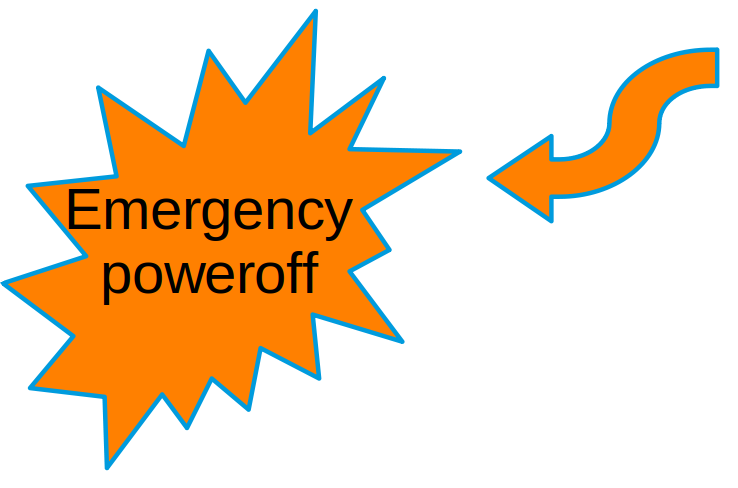
\includegraphics[width=1\linewidth]{img/isr/emergpoff.png}
	}
	\only<5->{
		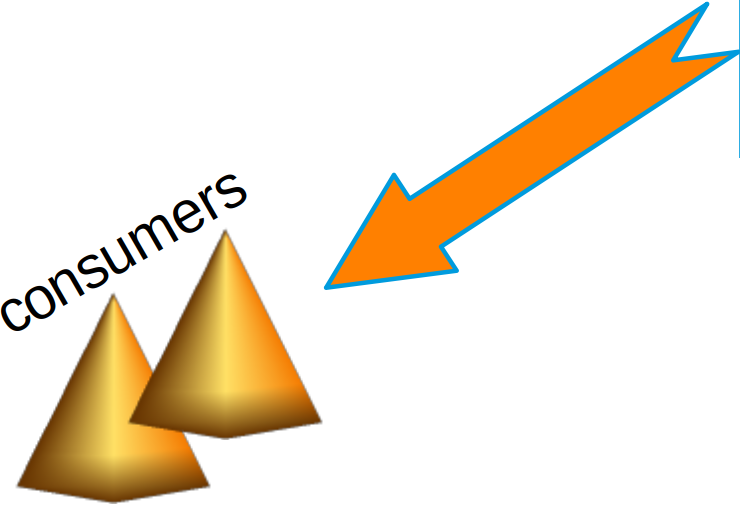
\includegraphics[width=1\linewidth]{img/isr/consumers.png}
	}
	\column[t]{0.25\linewidth}
	helper \\[4pt]
	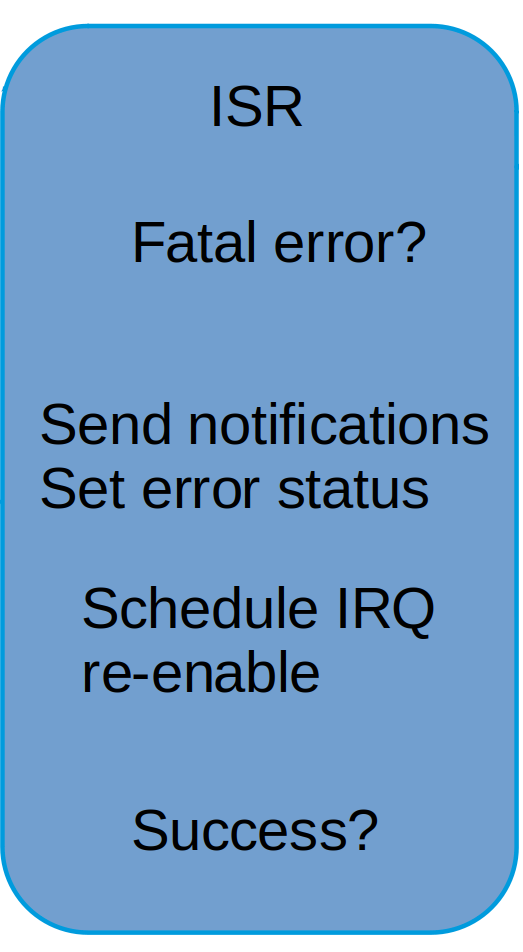
\includegraphics[width=1\linewidth]{img/isr/helperbox_size.png}
	\column[t]{0.20\linewidth}
	action \\[12pt]
	\only<3->{
		
\includegraphics[width=1\linewidth]{img/isr/map_event.png}
	}
	\only<4->{
		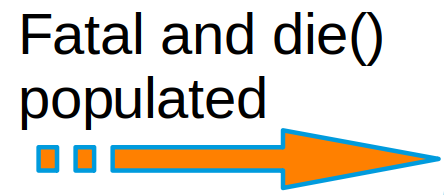
\includegraphics[width=1\linewidth]{img/isr/die.png}\vspace{20pt}
	}
	\only<6->{
		
\includegraphics[width=1\linewidth]{img/isr/renable.png}
	}
	\only<7->{
		
\includegraphics[width=0.5\linewidth]{img/isr/retry.png}
	}
	\column[t]{0.30\linewidth}
	driver \\[4pt]
	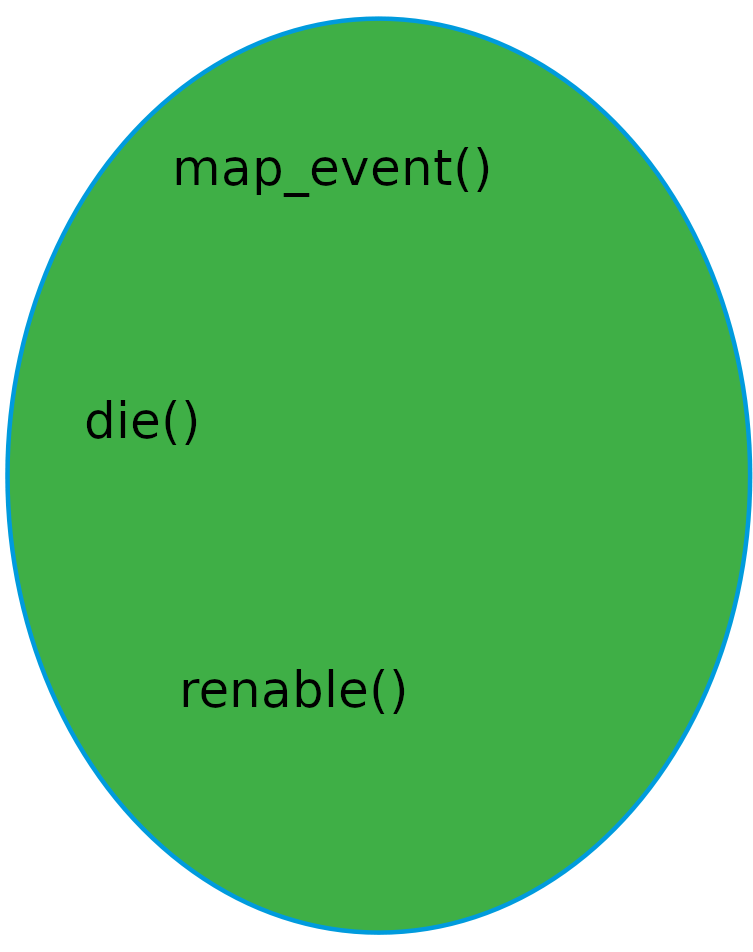
\includegraphics[width=1\linewidth]{img/isr/driver_size.png}
	\end{columns}
\end{frame}


%--------------  limit config callbacks page

\begin{frame}[fragile]{Helper configuration}
\note[item]<1>{Let's get back to helper registration.}
\note[item]<1>{Helper config information is given in struct regulator$\_$irq$\_$desc}
\note[item]<1>{fatal$\_$cnt can be used to mark failures to handle event as fatal. Eg. after checking this many  times for whether the condition is resolved (attempts to re-enable), die() is called or emergency power-off is executed}
\note[item]<2>{reread$\_$ms is time to wait after failed event mapping until retrying}
\note[item]<2>{irq$\_$off$\_$ms is time to keep IRQ disabled (before calling renable() if provided}
\note[item]<3>{skip$\_$off and high$\_$prio are something that were used in existing event implementations}
\note[item]<3>{skip$\_$off can be specified to not handle IRQs for regulators that are disabled}
\note[item]<3>{high$\_$prio can be set to use high$\_$priority work-queue for trying to re-enable the IRQ}
\note[item]<4>{data is pointer which can be used to store data needed in call-backs - like the driver private data}
\note[item]<4>{Callbacks for die(), mapping event and seeing if IRQ can be re-enabled. We will see the callbacks later}
\note[item]<5>{On top of this on the helper registration we provide}
\note[item]<5>{device pointer and IRQ information}
\note[item]<5>{errors that are common to all regulator devices this IRQ can be indicating errors for}
\note[item]<5>{errors specific to only some of the regulator devices}
\note[item]<5>{and finally an array of the regulator devices for which this IRQ can indicate problems}

\mycfile{include/linux/regulator/driver.h}
\lstset{language=C}
\scriptsize

\begin{lstlisting}
struct regulator_irq_desc {
	const char *name;
	int fatal_cnt;
 \end{lstlisting}
\pause
\begin{lstlisting}
	int reread_ms;
	int irq_off_ms;
 \end{lstlisting}
\pause
\begin{lstlisting}
	bool skip_off;
	bool high_prio;
 \end{lstlisting}
\pause
\begin{lstlisting}
	void *data;
	int (*die)(struct regulator_irq_data *rid);
	int (*map_event)(int irq, struct regulator_irq_data *rid,
	     unsigned long *dev_mask);
	int (*renable)(struct regulator_irq_data *rid);
};
 \end{lstlisting}
\pause

\begin{lstlisting}
void *regulator_irq_helper(struct device *dev,
		   const struct regulator_irq_desc *d, int irq,
		   int irq_flags, int common_errs, 
		   int *per_rdev_errs, struct regulator_dev **rdev,
		   int rdev_amount);
\end{lstlisting}
(or a devm-variant)
\end{frame}

%--------------  Event mapping page

\begin{frame}[fragile]{Event mapping}

\note[item]<1>{in order to find the reason for the IRQ, the helper is invoking a driver callback map$\_$event()}
\note[item]<1>{The driver should fill in what regulators were sending notification and what events/errors were detected}

\note[item]<2>{struct regulator$\_$irq$\_$data is used for this}
\note[item]<2>{contains array of regulator states for all regulators which can be informing events via this IRQ}
\note[item]<2>{number of the regulators}
\note[item]<2>{data pointer as was passed at helper registration}
\note[item]<2>{opaque integer. Mainly for delivering information about detected events to renable. Usually status register value which can be compared to see if situation has changed}

\note[item]<3>{The status for each regulator is filled in regulator$\_$err$\_$state struct}
\note[item]<3>{pointer to regulator device which state this struct is informing}
\note[item]<3>{notifs is the regulator notification flags}
\note[item]<3>{errors is the regulator error flags}
\note[item]<3>{possible$\_$errs should contain the errors this IRQ can be informing. Used to clear error statuses when re-enabling the IRQ}

\note[item]<4>{driver can provide a renable() call-back, which should be checking if reported problem has gone and IRQ can be re-enabled}
\note[item]<4>{gets a pointer to the same struct regulator$\_$irq$\_$data as map$\_$event() did}
\note[item]<4>{simplest for just checks current status register value and compares to the opaque value}
\note[item]<4>{it is possible there is some new errors - or some old have gone while some have stayed. In this case the renable may prefer indicating that IRQ should be enabled. This will probably yield a new IRQ and updated set of notifications to be sent}

\note[item]<5>{finally, for simple HW where an IRQ can only signal one type of errors, on one regulator, driver can use generic helper called regulator$\_$irq$\_$map$\_$event$\_$simple()}

\mycfile{include/linux/regulator/driver.h}
\lstset{language=C}
\scriptsize

\begin{lstlisting}
int (*map_event)(int irq, struct regulator_irq_data *rid,
		 unsigned long *dev_mask);
 \end{lstlisting}
\pause
\begin{lstlisting}
struct regulator_irq_data {
	struct regulator_err_state *states;
	int num_states;
	void *data;
	long opaque;
};
 \end{lstlisting}
\pause
\begin{lstlisting}
struct regulator_err_state {
	struct regulator_dev *rdev;
	unsigned long notifs;
	unsigned long errors;
	int possible_errs;
};
 \end{lstlisting}
\pause

\begin{lstlisting}
int (*renable)(struct regulator_irq_data *rid);
 \end{lstlisting}
\pause

\begin{lstlisting}
int regulator_irq_map_event_simple(int irq,
			struct regulator_irq_data *rid,
			unsigned long *dev_mask)
 \end{lstlisting}
\end{frame}

%--------------  Event mapping example

\begin{frame}[fragile]{Event mapping example}

\note[item]<1>{example of ROHM BD9576 over-voltage IRQ's event mapping function}
\note[item]<1>{This IRQ can be reporting over-voltage for voltage outputs 1 to 4}
\note[item]<1>{first the event mapping function reads the status from the hardware}
\note[item]<1>{if read fails, we return the REGULATOR$\_$FAILED$\_$RETRY}
\note[item]<1>{at the moment in BD9576 case the failures are not marked fatal though - eg, no number of failures will cause emergency power-off}

\note[item]<2>{The status is stored to the opaque data so that we can easily see if stauses have changed at renable()}
\note[item]<2>{dev$\_$mask is initialized. dev$\_$mask is a bit mask indicating which of the regulators in the status array are flagging problems}
\note[item]<2>{If no regulators were indicating problems, then we just return Ok}
\note[item]<3>{Else, we will be setting the bits for failing regulators. The BD9576 status register directly has this information in correct format (bit 0 maps to first regulator, bit 1 in second and so on)}
\note[item]<3>{finally, the notification and error flags are updated. The BD9576 uses same IRQ mechanism for WARNING and ERROR level notifications allowing the board designer to decide whether OVD should be treated as an ERROR or WARNING severity issue. The flags to advertise are then selected at probe time}

\mycfile{drivers/regulator/bd9576-regulator.c}
\lstset{language=C}
\scriptsize

\begin{lstlisting}
static int bd9576_ovd_handler(int irq, struct regulator_irq_data *rid,
			      unsigned long *dev_mask)
{
	ret = regmap_read(d->regmap, BD957X_REG_INT_OVD_STAT, &val);
	if (ret)
		return REGULATOR_FAILED_RETRY;

\end{lstlisting}

\pause
\begin{lstlisting}
	rid->opaque = val & OVD_IRQ_VALID_MASK;
	*dev_mask = 0;

	if (!(val & OVD_IRQ_VALID_MASK))
		return 0;
\end{lstlisting}
\pause
\begin{lstlisting}
	*dev_mask = val & BD9576_xVD_IRQ_MASK_VOUT1TO4;

	for_each_set_bit(i, dev_mask, 4) {
		stat  = &rid->states[i];

		stat->notifs	= rdata->ovd_notif;
		stat->errors	= rdata->ovd_err;
	}

	return 0;
}

\end{lstlisting}
\end{frame}


%--------------  Helper regisration example

\begin{frame}[fragile, t]{Helper registration 1/3}\vspace{4pt}

\note<1>{Helper registration. Let's look at relevant bits of BD9576 PMIC driver to see an exaple of helper registration for over-voltage}
\note[item]<1>{ Just read the intention and reveal the code block +  pause so people can understand the code}
\note[item]{name - obvious}
\note[item]{we keep IRQs disabled for a second}
\note[item]{We don't make this fatal or give a die() callback}
\note[item]{populate map$\_$event and renable}
\lstset{language=C}

\large Fill the helper configuration
\vfill
%\pause

\mycfile{drivers/regulator/bd9576-regulator.c}
%\scriptsize
\scriptsize
\begin{lstlisting}
static const struct regulator_irq_desc bd9576_notif_ovd = {              
       .name = "bd9576-ovd",                                            
       .irq_off_ms = 1000,                                              
       .map_event = bd9576_ovd_handler,                                 
       .renable = bd9576_ovd_renable,                                   
       .data = &bd957x_regulators,                                      
}; 
\end{lstlisting}
\end{frame}

\begin{frame}[fragile, t]{Helper registration 2/3}\vspace{4pt}

\note[item]{in a loop where we register regulators, we add regulators which can inform OVD to the ovd$\_$devs array}

\lstset{language=C}

\large Create an array of regulators this IRQ may concern
\vfill
%\pause
\mycfile{drivers/regulator/bd9576-regulator.c}

\scriptsize

\begin{lstlisting}
struct regulator_dev *ovd_devs[BD9576_NUM_OVD_REGULATORS];

for (i = 0; i < num_rdev; i++) {
	struct bd957x_regulator_data *r = &ic_data->regulator_data[i];
	const struct regulator_desc *desc = &r->desc;

	r->rdev = devm_regulator_register(&pdev->dev, desc, &config);

	rdevs[i] = r->rdev;
	if (i < BD957X_VOUTS1)
		ovd_devs[i] = r->rdev;
}
\end{lstlisting}
\end{frame}

\begin{frame}[fragile, t]{Helper registration 3/3}\vspace{4pt}
Fill possible errors this IRQ may indicate and register the helper
\vfill
\mycfile{drivers/regulator/bd9576-regulator.c}
\scriptsize

\begin{lstlisting}
int ovd_errs = REGULATOR_ERROR_OVER_VOLTAGE_WARN |
	 REGULATOR_ERROR_REGULATION_OUT;

ret = devm_regulator_irq_helper(&pdev->dev, &bd9576_notif_ovd,
				irq, 0, ovd_errs, NULL,
				&ovd_devs[0],
				BD9576_NUM_OVD_REGULATORS);

\end{lstlisting}
\end{frame}

%============== Section Wrap-up

\addtocounter{framenumber}{-1}
\begin{frame}[plain]
\section{Wrap it up}
\end{frame}

\begin{frame}{Summary}
\begin{itemize}
	\item Powering up a modern SOC is not simple
	\item PMIC is an IC trying to integrate powering related features into single chip
	\item Many PMICs include functional-safety features
	\item There is some existing support for indicating abnormal events
\end{itemize}
\end{frame}

\begin{frame}{No answers guaranteed}
\center
\only<1>{ \huge Questions?}
\only<2>{ \huge Thank You for listening! \\
(or time to wake up) :)}
\end{frame}

\addtocounter{framenumber}{-1}
\begin{frame}[fragile, plain]{Extras}
\lstset{language=C}
\scriptsize
How to handle notifications?
\begin{lstlisting}
typedef int (*notifier_fn_t)(struct notifier_block *nb,
			unsigned long action, void *data);

struct notifier_block {
	notifier_fn_t notifier_call;
	struct notifier_block __rcu *next;
	int priority;
};

/**
 * regulator_register_notifier - register regulator event notifier
 * @regulator: regulator source
 * @nb: notifier block
 *
 * Register notifier block to receive regulator events.
 */
int regulator_register_notifier(struct regulator *regulator,
                              struct notifier_block *nb) 
\end{lstlisting}
\end{frame}

\end{document}
